\subsection{Full robot description}
%
This section presents the kinematic model of the CLIO robot (see Fig. \ref{fig:3dmodel}). 
We model the robot as a serial kinematic chain with $n=9$ \gls{dofs} represented by the configuration vector $q \in \Rnum^n$. 
In the specific, we employ 2 \textit{passive} 
(rotational) joints to model the attachment interface between the anchor point (a fixed link) and the rope.
The rope is modeled as an \textit{actuated} prismatic joint ($q_{R}$), 
followed by 3 \textit{passive} rotational joints to model 
the connection between the rope and the \textit{base link} of the robot\footnote{It would be equivalent to allocate 3 joints at the anchor point and 2 at the base. 
To avoid redundancy in the representation, it is necessary  to have only one passive joint along the rope axis.}. 

The propulsion mechanism that allows the robot to jump is represented by a 3-DoF
robotic leg with a point-like foot that enables to exert a \textit{pure} Cartesian force (no moment) on the wall. 
The leg has two \textit{subsequent} rotational joints, called  hip pitch ($q_{HP}$ about the Y axis (green)) and hip 
roll ($q_{HR}$ about the X axis (red)), respectively. The joints are useful to align  the leg in the 
direction of the thrusting impulse. This enables to avoid to generate \textit{centroidal} moments that
 would initiate the pivoting of the robot around the Z axis (blue),  
 dealing with this is out of the scope of this paper (and part of future works). 
Finally a prismatic knee (($q_{K}$) joint is used to generate the \textit{thrusting} impulse. 
\footnote{With the actual design the robot will not be able to stabilize itself on the wall, 
	however the design of a landing and stabilization mechanism is out of the scope of this work
	where we focus mainly on the jump motion. }

%\begin{figure}
%	\centering
%	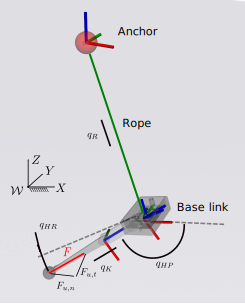
\includegraphics[width=0.7\columnwidth]{figs/3dmodel.pdf}
%	\caption{\small Kinematic model of the CLIO robot with  standard definitions. The anchor frame is aligned with an inertial ($\mathcal{W}$) frame.}
%	\label{fig:3dmodel}
%\end{figure}

The dynamics equation can be written as:  

\begin{align}
M (q) \ddot{q} + h(q,\dot{q}) = \mat{0_{5 \times 1} \\ \tau_a} + J^T F 
\end{align}

where $M \in \Rnum^{n \times n}$ is the inertia matrix; $h \in \Rnum^n$ represents the bias terms (Centrifugal, Coriolis and Gravity); and 
$J \in \Rnum^{3 \times n} $ is the Jacobian relative to the contact point mapping the contact force $F \in \Rnum^3$. 
Unless specified, all  vectors are expressed in an inertial $\mathcal{W}$ frame (attached to the anchor). 
The under-actuation is captured by the vector $0_{5 \times 1}$, while 
the efforts of the actuated joints are grouped into the vector $\tau_a = \mat{\tau_R & \tau_{\text{leg}}}^T \in \Rnum^4$.

\subsection{Simplified Model}
Dealing with the full dynamics of the robot can become intractable in an optimization setting, due to the 
high number of states and constraints involved. Therefore, in this section, we derive  a lower dimensional model 
(3 \gls{dofs}) that  captures the linear dynamics of the system, by making the following assumptions: 1) The mass is entirely concentrated in the body attached to the rope, 
2) we can unwind and rewind the rope that is assumed to be inextensible  rigid and remains completely elongated (i.e., it cannot bend), 
3) the rewinder mechanism can pull the rope when winding it but cannot push it (i.e., it can only act as a brake during the unwinding phase).
A geometric sketch of the system is shown in Fig. \ref{fig:sp} where the pitch angle is $\theta$, the yaw angle is $\phi$, 
and $l$ is the length of the rope. 

\begin{figure}
\centering
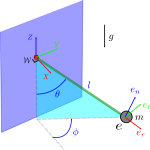
\includegraphics[width=0.8\columnwidth]{figs/simplifiedModel.pdf}
\caption{Logical scheme of the simplified model}
\label{fig:sp}
\end{figure}

Our input variables to the system are: 1) the rewinder pull action or
braking action $\mathbf{F}_r$ oriented along the rope, 2) an impulsive
pushing force $\mathbf{F}_u$ that the robot can generate when it is
attached to the mountain wall. 

Let $e$ be a frame attached to the point mass $m$, and let $\mathcal{W}$ be the world
frame attached to the anchor point of the pendulum.  If we
consider the homogeneous transformation from $e$ to $\mathcal{W}$, we can write: 
	\[
T_e^\mathcal{W} = \begin{bmatrix} R_z(\phi) & \mathbf{0}_{3 \times 1}  \\ \mathbf{0}_{1 \times 3}  & 1\end{bmatrix}  \begin{bmatrix} R_y( \frac{\pi}{2} - \theta) & \mathbf{0}_{3 \times 1}   \\ \mathbf{0}_{1 \times 3}  & 1\end{bmatrix}  
\begin{bmatrix} I_{3,3} &    \begin{matrix} l \\0 \\0 \end{matrix}    \\ \mathbf{0}_{1 \times 3}  & 1\end{bmatrix}  
	\]
Simplifying $T_e^\mathcal{W}$, gives 
	\[
	T_e^\mathcal{W} = \begin{bmatrix} c_\phi s_\theta & -s_\phi & c_\phi c_\theta & l c_\phi s_\theta\\
		s_\phi s_\theta & c_\phi & c_\theta s_\phi & l s_\phi s_\theta\\
		-c_\theta & 0 & s_\theta &-l c_\theta\\
		0 & 0 &0 &1\end{bmatrix} 
	\]		
where $c_x$ is a shorthand for $\cos x$ , and $s_x$ is a shorthand for $\sin x$.
The position $\mathbf{p}$ of the mass  can be extracted from the transformation matrix $T_\mathcal{B}^\mathcal{W}$ as: 
%
\begin{align}  
		\mathbf{p} &= \begin{bmatrix} x\\ y\\ z \end{bmatrix} =
		\begin{bmatrix}   
            l s_\theta c_\phi\\
			l s_\theta s_\phi\\
			-l c_\theta \end{bmatrix} \label{eq1}						
\end{align}

and the axes $e_r$, $e_t$, $e_n$ are the column of 	the top-left sub-matrix of $T_e^\mathcal{W}$, respectively.
%\begin{align}
%	\mathbf{e}_r &= \mat{	c_\phi s_\theta\\
%		s_\phi s_\theta\\
%		-c_\theta} \quad 
%	\mathbf{e}_t = \mat{-s_\phi\\
%		c_\phi\\
%		0} \quad 
%	\mathbf{e}_n = \mat{c_\phi c_\theta \\
%		s_\phi c_\theta\\
%		s_\theta}		
%\end{align}

%From equation \ref{eq1}, we can compute the velocities and the kinetic energy:   
From equation \eqref{eq1}, the velocities along the Cartesian axes are:
%
\begin{align*}
	\dot{x} &= 
	l c_\theta c_\phi \dot{\theta} - l s_\theta s_\phi \dot{\phi} + s_\theta c_\phi \dot{l} \\
	\dot{y} &= l c_\theta s_\phi \dot{\theta} + l s_\theta c_\phi \dot{\phi} + s_\theta s_\phi \dot{l} \\
	\dot{z} &= l s_\theta  \dot{\theta} - c_\theta \dot{l} 
\end{align*}
%
Next, the velocity of the mass squared:
\begin{align*}
	v^2 &= \dot{x}^2 + \dot{y}^2 + \dot{z}^2 =  l^2 \dot{\theta}^2 + l^2 s_\theta^2 \dot{\phi}^2 + \dot{l}^2 		
%	&=  l^2 \dot{\theta}^2 + l^2 s_\theta^2 \dot{\phi}^2 + \dot{l}^2\\
\end{align*}
%
Thus, the kinetic energy $K$ and potential energy $V$:  
%
\begin{align*}
	K &=\frac{ m }{2} v^2 =  \frac{m}{2} l^2 \left(\dot{\theta}^2 + s_\theta^2 \dot{\phi}^2 \right) + \frac{m }{2} \dot{l}^2  \\
    V &= mgz = -mgl c_\theta   \label{eq3}
\end{align*}
%
which leads to the Lagrangian function described as:
%
\begin{equation}
	L = K - V = \frac{m}{2} l^2 \left(\dot{\theta}^2 + s_\theta^2 \dot{\phi}^2\right) + \frac{m}{2}\dot{l}^2 + mgl c_\theta
\end{equation}
%
The dynamics of the system will be obtained using the Euler-Lagrange equation:




%%%%%%%%
%%
%\[
%\frac{d}{dt}\frac{\partial L}{\partial \dot{q}_i} - \frac{\partial L}{\partial q_i} = Q_i^p 
%\]
%where $Q_i^p$ is the generalized force along the $q_i$ generalized coordinate: 
%$Q_i^p = (\mathbf{F}_r + \mathbf{F}_u)  \frac{\partial \mathbf{p}}{\partial q_i}$ , \\
%$\mathbf{F}_r$ is oriented along the rope ($\mathbf{e}_r$) and $\mathbf{F}_u$ is generated so that it does not have any component along the rope:
%%		
%\begin{equation}
%	\begin{aligned}
%		\mathbf{F}_r  &= F_r \mathbf{e}_r= F_r \begin{bmatrix}
%			c_\phi s_\theta\\
%			s_\phi s_\theta\\
%			-c_\theta
%		\end{bmatrix}  \\	
%		\mathbf{F}_u &= F_{u,t}\mathbf{e}_t + F_{u,n} \mathbf{e}_n = F_{u,t}
%		\begin{bmatrix}
%			-s_\phi\\
%			c_\phi\\
%			0
%		\end{bmatrix} + 
%		F_{u,n} \begin{bmatrix}
%			c_\phi c_\theta \\
%			s_\phi c_\theta\\
%			s_\theta
%		\end{bmatrix} 
%	\end{aligned}
%	\label{eq:forces}
%\end{equation}
%%
%Let the generalized coordinates $q_i$ be chosen as $q_1 = \theta$, $q_2 = \phi$ and $q_3 = l$. The corresponding velocities are:
%%
%\begin{align*}
%	\qquad	\frac{\partial \mathbf{p}}{\partial q_1} = \frac{\partial \mathbf{p}}{\partial \theta} &= \begin{bmatrix}
%			l c_\phi c_\theta\\
%			l s_\phi c_\theta\\
%			l s_\theta
%		\end{bmatrix},  \text{and} \quad 
%		\frac{\partial \mathbf{p}}{\partial q_2} = \frac{\partial \mathbf{p}}{\partial \phi} &= \begin{bmatrix}
%			- l s_\phi s_\theta\\
%			l c_\phi s_\theta\\
%			0
%		\end{bmatrix}, \\
%		\frac{\partial \mathbf{p}}{\partial q_3} = \frac{\partial \mathbf{p}}{\partial l} &= \begin{bmatrix}
%			c_\phi s_\theta\\
%			s_\phi s_\theta\\
%			-c_\theta
%		\end{bmatrix} .
%	\end{align*}
%
%	Hence,
%\begin{align*}
%	Q_1^p &= \left(\mathbf{F}_r + \mathbf{F}_u\right)   \frac{\partial \mathbf{p}}{\partial q_1} 
%	%% 		&= F_r \mathbf{f}_r \cdot  \frac{\partial \mathbf{p}}{\partial \theta} + \\
%	%% 		&+ F_{u,t} \mathbf{f}_{u,t} \cdot  \frac{\partial \mathbf{p}}{\partial \theta} + \\
%	%% 		&+ F_{u,n} \mathbf{f}_{u,n} \cdot  \frac{\partial \mathbf{p}}{\partial \theta}  =  \\
%	%% 		&= F_{u,n} \mathbf{f}_{u,n} \cdot  \frac{\partial \mathbf{p}}{\partial \theta} = \\
%	= F_{u,n} l , \\
%	% 	\end{align*}
%% 	\begin{align*}
%	Q_2^p &= \left(\mathbf{F}_r + \mathbf{F}_u\right)   \frac{\partial \mathbf{p}}{\partial q_2}
%	%% 		&= F_r \mathbf{f}_r \cdot  \frac{\partial \mathbf{p}}{\partial \phi} + \\
%	%% 		&+ F_{u,t} \mathbf{f}_{u,t} \cdot  \frac{\partial \mathbf{p}}{\partial \phi} + \\
%	%% 		&+ F_{u,n} \mathbf{f}_{u,n} \cdot  \frac{\partial \mathbf{p}}{\partial \phi}   = \\
%	%% 		&= F_{u,t} \mathbf{f}_{u,t} \cdot  \frac{\partial \mathbf{p}}{\partial \phi} =\\
%	= F_{u,t} l s_\theta,\\
%	%% 	\end{align*}
%%% 	\begin{align*}
%	Q_3^p &= \left(\mathbf{F}_r + \mathbf{F}_u\right)   \frac{\partial \mathbf{p}}{\partial q_3}
%	%% 		&= F_r \mathbf{f}_r \cdot  \frac{\partial \mathbf{p}}{\partial l} + \\
%	%% 		&+ F_{u,t} \mathbf{f}_{u,t} \cdot  \frac{\partial \mathbf{p}}{\partial l} + \\
%	%% 		&+ F_{u,n} \mathbf{f}_{u,n} \cdot  \frac{\partial \mathbf{p}}{\partial l}   = \\
%	%% 		&= F_r \mathbf{f}_r \cdot  \frac{\partial \mathbf{p}}{\partial l} =\\
%	= F_{r} .
%\end{align*}
%The Euler-Lagrange equations gives us, with the defined generalized coordinates, the non-linear dynamic equations of the system: 

% 	\begin{align*}
%		&\frac{d}{dt}\left(\frac{\partial L}{\partial \dot{\theta}} \right) - \frac{\partial L}{\partial \theta} = Q_1^p  \rightarrow  \\
%%		& \frac{d}{dt}\left(m l^2 \dot{\theta}\right) - (m l^2 s_\theta c_\theta \dot{\phi}^2 - m g l s_\theta) = F_{u,n}  l \\ 
 %		  &m l^2 \ddot{\theta} + 2 m l \dot{\theta} \dot{l} - m l^2 s_\theta c_\theta \dot{\phi}^2 + m g l s_\theta = F_{u,n} . l\\
%% 		& \ddot{\theta} + \frac{2}{l} \dot{\theta} \dot{l} - c_\theta s_\theta \dot{\phi}^2 + \frac{g}{l}  s_\theta =  \frac{F_{u,n}  }{ml}    
%% 	\end{align*}
%% 	The second Euler-Lagrange equation yields
%% 	\begin{align*}
%% 		&\frac{d}{dt}\left(\frac{\partial L}{\partial \dot{\phi}} \right) - \frac{\partial L}{\partial \phi} = Q_2^p    \\
%% 		&\frac{d}{dt}\left(m l^2 s_\theta^2 \dot{\phi}\right) = F_{u,t}  l  s_\theta\\
% 		 &\ddot{\phi} ml^2 s^2_\theta + 2 m l \dot{l} s_\theta^2 \dot{\phi} + 2 m l^2 s_\theta c_\theta \dot{\theta} \dot{\phi}  = F_{u,t}  l  s_\theta\\
%%		&\ddot{\phi} + 2 \frac{c_\theta}{s_\theta} \dot{\theta} \dot{\phi} + \frac{2}{l} \dot{\phi} \dot{l} = \frac{F_{u,t}}{ml s_\theta}
%% 	\end{align*}
%% 	The third Euler-Lagrange equation is as follows:
%% 	\begin{align*}
%% 		&\frac{d}{dt}\left(\frac{\partial L}{\partial \dot{l}} \right) - \frac{\partial L}{\partial l} = Q_3^p    \\
%% 		&\frac{d}{dt}\left(m\dot{l}\right) - (m l \dot{\theta}^2 + m l s^2_\theta \dot{\phi}^2 + m g c_\theta) = F_r ,
% 		&m \ddot{l} - m l \dot{\theta}^2 - m l s^2_\theta \dot{\phi}^2 - m g c_\theta = F_r 
%% 		&\ddot{l} - l \dot{\theta}^2 - l s^2_\theta \dot{\phi}^2 - g c_\theta = \frac{F_r}{m} 
 %	\end{align*}
           %%
        
%Overall, the non-linear dynamic equations of the system 
\begin{equation}
\begin{aligned}
		&\ddot{\theta} + \frac{2}{l} \dot{\theta} \dot{l} - c_\theta s_\theta  \dot{\phi}^2 + \frac{g}{l}  s_\theta =  \frac{1}{ml}F_{u,n} \\
		&\ddot{\phi} + 2 \frac{c_\theta}{s_\theta} \dot{\theta} \dot{\phi} + \frac{2}{l} \dot{\phi} \dot{l} = \frac{1}{ml s_\theta} F_{u,t} \\
		&\ddot{l} - l \dot{\theta}^2 - l s^2_\theta \dot{\phi}^2 - g c_\theta = \frac{1}{m} F_r .
\end{aligned}
\label{eq:nonlinearDyn}
\end{equation}

        Clearly, in this derivation of the model, we have heavily
        relied on the point-mass nature of the body.  A possible issue
        could be the rotational dynamics of the body around the rope axis,
        which could waste energy generating unnecessary motions and
        impede the landing phase. This issue will be part of our
        future work. However, as discussed next, under reasonable
        assumptions (e.g., thrusting force oriented in the direction
        of the center of mass), the results based on the simplified
        model can be applied to a realistic system with a good approximation.

\subsection{Robot motion: problems and solution overview}
The problem of moving CLIO between two given configurations is not 
easy.  First of all, even the simplified dynamics in~\eqref{eq:nonlinearDyn} is highly nonlinear.  Second, 
the configurations the robot moves between can in general be 
distant, and therefore it is not possible to
use the linearized dynamics.  Third, one of our
actuators, the thrusting force $\mathbf{F}_u$, has an impulsive nature
and operates at discrete time instants. Therefore, it is not possible
to use it in any feedback control scheme.
Finally, the tangential component $F_{u,t}$ is generated by
using friction. Therefore, the two components $F_{u,n}$ and $F_{u,t}$ are coupled
by the nonlinear friction cone constraints. Because the friction cone
depends on the specific point or area where the robot is pointing its leg,
this mechanism is not totally reliable (i.e., there can be significant deviations
between generated and desired values of $F_{u,t}$).

In view of this complexity, we propose an approach based on two steps:
1. a motion strategy is planned prior to starting the motion,
2. after take off, a feedback motion controller operates on
$\mathbf{F}_r$ to compensate for small deviations and
secure that the robot lands close to the expected position.

